\section{Extracción de información}

\subsection{Extracción}

Imaginemos que tenemos un log de la forma
$$
    \begin{array}{lll}
        \texttt{18:30} & \texttt{ ERROR 06} \\
        \texttt{19:10} & \texttt{ OK 00}    \\
        \texttt{20:00} & \texttt{ ERROR 19}
    \end{array}
$$
y queremos obtener todas las horas $\texttt{HH:MM}$, quizá con una expresión regular $R =$ ({\textbackslash}d{\textbackslash}d:{\textbackslash}d{\textbackslash}d). ¿Cómo podemos \textbf{automatizar} esta tarea de extraer datos?
\begin{enumerate}
    \item Una tarea como la anterior \textbf{se puede programar fácilmente}, ¿por qué queremos automatizarla?
    \item Las expresiones regulares ya hacen el trabajo anterior, ¿por qué queremos \textbf{estudiar este problema de nuevo}?
\end{enumerate}
En esta última sección veremos \textbf{nuevas técnicas formales y algorítmicas} para entender y resolver este problema.

\subsubsection{Spans}

\paragraph{Definición.} Para un documento $d = a_0 a_1 \ldots a_{n-1}$ se define un \textbf{span} $s$ de $d$ como:
\alignformula{
s=[i, j\rangle
}
tal que $0 \leq i \leq j \leq n$. \bigbreak

Si $s = [i,j \rangle$ es un span de $d$ se define:
\alignformula{
d[s]=d[[i, j\rangle]=a_i a_{i+1} \ldots a_{j-1}
}
como el \textbf{contenido del span} $s$ en $d$. Si $i = j$, entonces $d[[i, i\rangle]=\epsilon$.
\ejemplo{}{}{
    \vspace{-10pt}
    \img{img/cap6/ejemplo1.png}{0.4}
}

Denotamos el conjunto de \textbf{todos los spans} de $d$ como $\texttt{Spans}(d)$.

\newpage
\subsubsection{Regex}
\paragraph{Sintaxis.} Sea $\Sigma$ un alfabeto finito y $\ca{X}$ un conjunto de variables. $R$ es una expresión regular con variables (o \textbf{regex}) sobre $\Sigma$ si $R$ es igual a:
\begin{enumerate}
    \item $a$, para alguna letra $a \in \Sigma$.
    \item $\epsilon$
    \item $\mathbf{x}\{R_1\}$, donde $R_1$ es una regex y $\mathbf{x} \in X$.
    \item $(R_1 + R_2)$, donde $R_1$ y $R_2$ son regex.
    \item $(R_1 \cdot R_2)$, donde $R_1$ y $R_2$ son regex.
    \item $(R_1^*)$, donde $R_1$ es una regex.
\end{enumerate}

$\mbb{x}\{R_1\}$ representa que el \textbf{span capturado} por $R_1$ lo almacenaremos en la variable $\mbb{x}$.

\ejemplo{}{}{
    Sea $\Sigma = \{a,b,\sbar\}$.
    \begin{itemize}
        \item $\Sigma^* \cdot \mbb{x}\{abba\} \cdot \Sigma^*$
        \item $\Sigma^* \cdot \sbar \cdot \mbb{x}\{ab \cdot (a+b)^*\}\cdot \sbar \cdot \Sigma^*$
        \item $\Sigma^* \cdot \sbar \cdot \mbb{x}\{(a+b)^*\}\cdot \sbar \cdot \mbb{y}\{(a+b)^*\} \cdot \sbar \cdot \Sigma^*$
        \item $(\Sigma^* \cdot \sbar + \epsilon) \cdot \mbb{z}\{\mbb{x}\{(a+b)^+\}\cdot \sbar \cdot \mbb{y}\{(a+b)^+\}\} \cdot (\epsilon + \sbar \cdot \Sigma^*)$
        \item $\Sigma^* \cdot \mbb{x}\{abba\} \cdot \sbar \cdot \mbb{x}\{baba\} \cdot \Sigma^*$
    \end{itemize}
}

\paragraph{Regex válidas.} Sea $\texttt{Var}(R)$ el conjunto de \textbf{todas las variables} en $\ca{X}$ mencionadas en $R$. Decimos que $R$ es una regex \textbf{válida} si, y sólo si, todas las siguientes condiciones se cumplen:
\begin{enumerate}
    \item si $R = R_1 \cdot R_2$, entonces $\texttt{Var}(R_1) \cap \texttt{Var}(R_2) = \varnothing$, y $R_1$ y $R_2$ son válidas.
    \item si $R = R_1 + R_2$, entonces $\texttt{Var}(R_1) = \texttt{Var}(R_2)$, y $R_1$ y $R_2$ son válidas.
    \item si $R = R_1^*$, entonces $\texttt{Var}(R_1) = \varnothing$, y $R_1$ es válida.
    \item si $R = \mbb{x}\{R_1\}$, entonces $\mbb{x} \notin \texttt{Var}(R_1)$, y $R_1$ es válida.
\end{enumerate}

Si $R$ es \textbf{válida} nos permite asignar las variables de \textbf{manera correcta}.

\ejemplo{}{}{
    Las siguientes regex son válidas:
    \begin{itemize}
        \item $\Sigma^* \cdot \mbb{x}\{abba\} \cdot \Sigma^*$
        \item $\Sigma^* \cdot \mbb{x}\{abba\} \cdot \sbar \cdot \mbb{y}\{baba\} \cdot \Sigma^*$
        \item $\Sigma^* \cdot \sbar \cdot \mbb{x}\{ab\cdot (a+b)^*\} \cdot \sbar \cdot \Sigma^*$
    \end{itemize}
    Las siguientes regex \textbf{no} son válidas:
    \begin{itemize}
        \item $\Sigma^* \cdot \mbb{x}\{abba\} \cdot \sbar \cdot \mbb{x}\{baba\} \cdot \Sigma^*$
        \item $\Sigma^* \cdot (\mbb{x}\{abba\} + \mbb{y}\{baba\}) \cdot \Sigma^*$
        \item $\Sigma^* \cdot \sbar \cdot (\mbb{x}\{ab \cdot (a+b)^*\} \cdot \sbar)^* \cdot \Sigma^*$
    \end{itemize}
}

\paragraph{Mappings.} Un \textbf{mapping} de $R$ sobre un documento $d \in \Sigma^*$ es una función:
\alignformula{
    \mu: \texttt{Var}(R) \to \texttt{Spans}(d)
}

donde el dominio de $\mu$ es $\texttt{dom}(\mu) = \texttt{Var}(R)$. \bigbreak

Se define el mapping $\mu = \, \perp$ como el \textbf{mapping vacío} donde $\texttt{dom}(\perp) = \varnothing$.

\ejemplo{}{}{
    \img{img/cap6/ejemplo4.png}{0.3}
}

\begin{itemize}
    \item Para una variable $\mbb{x}$ y span $s$ se define el \textbf{mapping} de una variable:
          $$
              \mu=[\mathbf{x} \mapsto s] \quad \text { tal que } \quad \texttt{dom}(\mu)=\{\mathbf{x}\} \quad \text { y } \quad \mu(\mathbf{x})=s
          $$

    \item Para $k \in \mathbb{N}$ se define el \textbf{mapping} $\mu + k$ tal que $\texttt{dom}(\mu + k) = \texttt{dom}(\mu)$ y:
          $$
              \text{si } \mu(\mathbf{x})=[i, j\rangle \text { entonces }[\mu+k](\mathbf{x})=[i+k, j+k\rangle \text {.}
          $$

    \item Para mappings $\mu_1,\mu_2$ con $\texttt{dom}(\mu_1) \cap \texttt{dom}(\mu_2) = \varnothing$ se define la \textbf{unión}:
          $$
              \mu=\mu_1 \cup \mu_2 \quad \text { tal que } \quad \mu(\mathbf{x})= \begin{cases}
                  \mu_1(\mathbf{x}) & \text { si } \mathbf{x} \in \operatorname{dom}\left(\mu_1\right) \\
                  \mu_2(\mathbf{x}) & \text { si } \mathbf{x} \in \operatorname{dom}\left(\mu_2\right)
              \end{cases}
          $$
\end{itemize}

\paragraph{Semántica regex.} Para una regex válida $R$ cualquiera, se define la función $\llbracket R \rrbracket$ \textbf{inductivamente} sobre documentos $d \in \Sigma^*$:
\begin{enumerate}
    \item $\llbracket a \rrbracket(d)=\{\perp\}$ si $d = a$, y $\varnothing$ en otro caso.
    \item $\llbracket \epsilon \rrbracket(d)=\{\perp\}$ si $d = \epsilon$, y $\varnothing$ en otro caso.
    \item $\llbracket \mathbf{x}\left\{R_1\right\} \rrbracket(d)=\left\{\mu \cup[\mathbf{x} \mapsto s] \mid \mu \in \llbracket R_1 \rrbracket(d) \text { y } s=[0,|d|\rangle\right\}$
    \item $\llbracket R_1 \cdot R_2 \rrbracket(d)=\left\{\begin{array}{l|l}
                  \mu_1 \cup\left(\mu_2+\left|d_1\right|\right) & \begin{array}{l}
                                                                      \text { existe } d_1, d_2 \text { tal que } d=d_1 \cdot d_2, \\
                                                                      \mu_1 \in \llbracket R_1 \rrbracket\left(d_1\right) \text { y } \mu_2 \in \llbracket R_2 \rrbracket\left(d_2\right)
                                                                  \end{array}
              \end{array}\right\}$

          Como $R_1 \cdot R_2$ son válidas, entonces sabemos que $\texttt{dom}(\mu_1) \cap \texttt{dom}(\mu_2) = \varnothing$.

    \item $\llbracket R_1+R_2 \rrbracket(d)=\llbracket R_1 \rrbracket(d) \cup \llbracket R_2 \rrbracket(d)$

    \item $\llbracket R_1^* \rrbracket(d)=\bigcup_{k=0}^{\infty} \llbracket\left(R_1\right)^k \rrbracket(d)$

          Como $\texttt{Var}(R_1) = \varnothing$, entonces $\llbracket R_1^* \rrbracket(d)=\{\perp\}$ si, y sólo si, $d \in \mathcal{L}\left(R_1^*\right)$.
\end{enumerate}

\ejemplo{}{}{
    \begin{itemize}
        \item $\llbracket b \rrbracket(a) = \varnothing$
        \item $\llbracket b \rrbracket(b) = \{\perp\}$
        \item $\llbracket \mbb{x}\{b\} \rrbracket(a) = \varnothing$
        \item $\llbracket \mbb{x}\{b\} \rrbracket(b) = \{ [\mbb{x} \mapsto [0,1\rangle] \}$
        \item $\llbracket \mathbf{x}\{b\} b \rrbracket(b b)=\{[\mathbf{x} \mapsto[0,1\rangle]\}$
        \item $\llbracket b \mathbf{x}\{b\}\rrbracket(b b)=\{[\mathbf{x} \mapsto[1,2\rangle]\}$
        \item $\llbracket\mathbf{x}\{b\} \mathbf{y}\{b\}\rrbracket(b b)=\{[\mathbf{x} \mapsto[0,1\rangle, \mathbf{y} \mapsto[1,2\rangle]\}$
        \item $\llbracket\mathbf{x}\{b\} b+b \mathbf{x}\{b\}\rrbracket(b b)=\{[\mathbf{x} \mapsto[0,1\rangle],[\mathbf{x} \mapsto[1,2\rangle]\}$
    \end{itemize}
}

\ejemplo{}{}{
    \vspace{-10pt}
    \img{img/cap6/ejemplo6.png}{0.5}

    \begin{itemize}

        \item $\llbracket\Sigma^* \cdot \mathbf{x}\{a b a+b a b\} \cdot \Sigma^*\rrbracket(d)=\{[\mathbf{x} \mapsto[10,13\rangle],[\mathbf{x} \mapsto[11,14\rangle]\}$

        \item $\llbracket\Sigma^* \cdot \sbar \cdot \mathbf{x}\left\{b a \cdot(a+b)^*\right\} \cdot \sbar \cdot \Sigma^*\rrbracket(d)=\{[\mathbf{x} \mapsto[7,9\rangle],[\mathbf{x} \mapsto[10,14\rangle]\}$

        \item $\llbracket\Sigma^* \cdot \mathbf{x}\{a b b a\} \cdot \sbar \cdot \mathbf{y}\{b a\} \cdot \Sigma^*\rrbracket(d)=\{[\mathbf{x} \mapsto[2,6\rangle, \mathbf{y} \mapsto[7,9\rangle]\}$

        \item $\llbracket\Sigma^* \cdot \sbar \cdot \mathbf{x}\left\{(a+b)^*\right\} \cdot \sbar \cdot \mathbf{y}\left\{(a+b)^*\right\} \cdot \sbar \cdot \Sigma^*\rrbracket(d)=\{[\mathbf{x} \mapsto[2,6\rangle, \mathbf{y} \mapsto[7,9\rangle],[\mathbf{x} \mapsto[7,9\rangle, \mathbf{y} \mapsto[10,14\rangle]\}$

        \item $\llbracket\Sigma^* \cdot \mathbf{x}\left\{\Sigma^*\right\} \cdot \Sigma^* \rrbracket(d)=\texttt{Spans}(d)$

    \end{itemize}
}

\paragraph{Evaluación regex.} Podemos preguntarnos:

\begin{itemize}
    \item Dado una regex $R$ con una variable, ¿de qué tamaño puede ser $|\llbracket R \rrbracket(d)|$ con respecto a $|d|$ \textbf{en el peor caso}?
    \item Dado una regex $R$ con $k$ variables, ¿de qué tamaño puede ser $|\llbracket R \rrbracket(d)|$ con respecto a $|d|$ y $k$ \textbf{en el peor caso}?
\end{itemize}

La respuesta es que el tamaño de $|\llbracket R \rrbracket(d)|$ puede crecer de manera exponencial. ¿Cómo podemos evaluar entonces una regex de $R$ \textbf{eficientemente}? Analizamos una herramienta para lograr esto a continuación/

\subsubsection{Vset autómata}

¿Qué tiene de nuevo un autómata con variables (vset autómata)?
\begin{enumerate}
    \item Tiene transiciones con \textbf{abre} y \textbf{cierra} de variable $\mbb{x}$:
          \alignformula{
              p \stackrel{\langle x}{\rightarrow} q \quad y \quad p \stackrel{x\rangle}{\rightarrow} q
          }
    \item Cada ejecución define un \textbf{mapping} de las variables a spans.
\end{enumerate}
Un \textbf{vset autómata} será nuestro primer modelo para \textbf{compilar regex}.

\paragraph{Definición.} Un vset autómata (VA) es una tupla:
\alignformula{
    \ca{A} = (Q, \Sigma, \ca{X}, \Delta, I, F)
}
\begin{itemize}
    \item $Q$ es un conjunto fifnito de estados.
    \item $\Sigma$ es el alfabeto de input.
    \item $\ca{X}$ es un conjunto finito de variables.
    \item $\Delta \subseteq Q \times(\Sigma \cup\{\epsilon\} \cup\{\langle\mathbf{x}, \mathbf{x}\rangle \mid \mathbf{x} \in \mathcal{X}\}) \times Q$ es la relación de transición.
    \item $I \subseteq Q$ es un conjunto de estados iniciales.
    \item $F \subseteq Q$ es el conjunto de estados finales (o aceptación).
\end{itemize}

`$\langle \mbb{x}$' simboliza \textbf{abrir} y `$\mbb{x}\rangle$' simboliza \textbf{cerrar} la variable $\mbb{x}$.

\ejemplo{vset autómatas}{}{
    \begin{figure}[H]
        \centering
        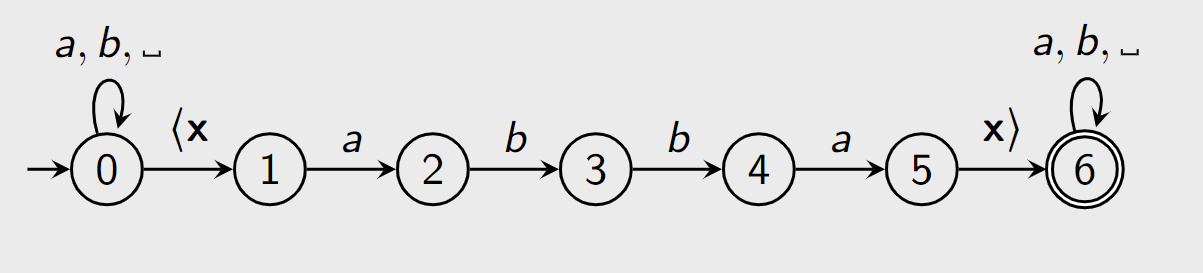
\includegraphics[scale=0.45]{img/cap6/ejemplo7_1.png}
        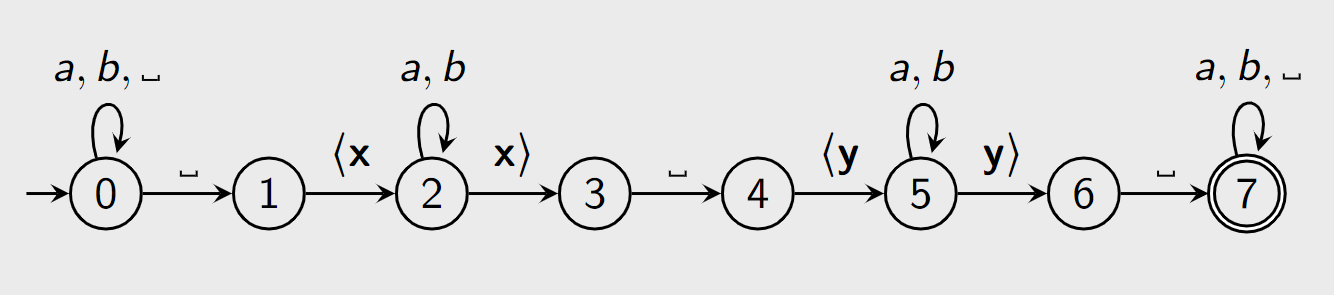
\includegraphics[scale=0.45]{img/cap6/ejemplo7_2.png}
        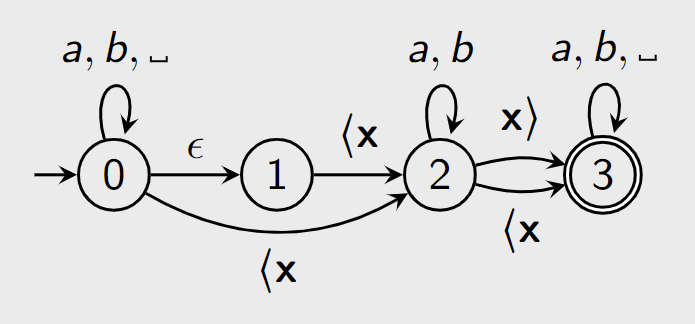
\includegraphics[scale=0.45]{img/cap6/ejemplo7_3.png}
    \end{figure}
}

\paragraph{Ejecución.} Sea $\ca{A} = (Q,\Sigma,\ca{X},\Delta,I,F)$ un VA y $d = a_0 \ldots a_{n-1} \in \Sigma^*$ un documento. Tenemos que:
\begin{itemize}
    \item Un par $(p, i) \in Q \times\{0, \ldots, n\}$ es una \textbf{configuración} de $\ca{A}$ sobre $d$.
    \item Una configuración $(p,0)$ es \textbf{inicial} si $q \in I$.
    \item Una configuración $(p, |d|)$ es \textbf{final} si $q \in F$.
\end{itemize}
\textit{``Intuitivamente, una configuración $(p,i)$ representa que $\ca{A}$ se encuentra en el estado $p$ antes de leer $a_i$''.} \bigbreak

Una \textbf{ejecución} (o \textit{run}) $\rho$ de $\ca{A}$ sobre $d$ es una secuencia:
\alignformula{
    \rho:\left(p_0, i_0\right) \stackrel{o_1}{\rightarrow}\left(p_1, i_1\right) \stackrel{o_2}{\rightarrow} \ldots \stackrel{o_m}{\rightarrow}\left(p_m, i_m\right)
}
tal que cumple todas las siguientes condiciones:
\begin{itemize}
    \item $o_k \in \Sigma \cup\{\epsilon\} \cup\{\langle\mathbf{x}, \mathbf{x}\rangle \mid \mathbf{x} \in \mathcal{X}\}$ con $k \leq m$,
    \item $(p_0, i_0)$ es una configuración inicial,
    \item para todo $k < m$, $\left(p_k, o_{k+1}, p_{k+1}\right) \in \Delta$,
    \item para todo $k \leq m$, si $o_k \in \Sigma$, entonces $o_k = a_{i_{k-1}}$ y $i_k = i_{k-1} + 1$,
    \item para todo $k \leq m$, si $o_k \in\{\epsilon\} \cup\{\langle\mathbf{x}, \mathbf{x}\rangle \mid \mathbf{x} \in \mathcal{X}\}$, entonces $i_k = i_{k-1}$.
\end{itemize}

Una ejecución $\rho$ es de \textbf{aceptación} si $(p_m, i_m)$ es de aceptación.

\ejemplo{Ejecuciones}{}{
    \img{img/cap6/ejemplo8.png}{0.5}
    Algunas ejecuciones sobre $d$:
    \begin{itemize}
        \item $\rho_1:\left(p_0, 0\right) \stackrel{a}{\rightarrow}\left(p_0, 1\right) \stackrel{b}{\rightarrow}\left(p_0, 2\right) \stackrel{a}{\rightarrow}\left(p_0, 3\right)$
        \item $\rho_2:\left(p_0, 0\right) \stackrel{a}{\rightarrow}\left(p_0, 1\right) \stackrel{\epsilon}{\rightarrow}\left(p_1, 1\right) \stackrel{\langle x}{\rightarrow}\left(p_2, 1\right) \stackrel{b}{\rightarrow}\left(p_2, 2\right) \stackrel{\mathrm{x}\rangle}{\rightarrow}\left(p_3, 2\right) \stackrel{a}{\rightarrow}\left(p_3, 3\right)$
        \item $\rho_3:\left(p_0, 0\right) \stackrel{a}{\rightarrow}\left(p_0, 1\right) \stackrel{\langle x}{\rightarrow}\left(p_2, 1\right) \stackrel{b}{\rightarrow}\left(p_2, 2\right) \stackrel{\mathrm{x}\rangle}{\rightarrow}\left(p_3, 2\right) \stackrel{a}{\rightarrow}\left(p_3, 3\right)$
        \item $\rho_4:\left(p_0, 0\right) \stackrel{a}{\rightarrow}\left(p_0, 1\right) \stackrel{\langle x}{\rightarrow}\left(p_2, 1\right) \stackrel{b}{\rightarrow}\left(p_2, 2\right) \stackrel{\langle x}{\rightarrow}\left(p_3, 2\right) \stackrel{a}{\rightarrow}\left(p_3, 3\right)$
    \end{itemize}

    Donde $\rho_2$ y $\rho_3$ son ejecuciones válidas.
}

Una ejecución $\rho$ es \textbf{válida} si, y sólo si, para todo $\mbb{x} \in \ca{X}$:
\begin{itemize}
    \item existe un único $k_1 \leq m$ tal que $o_{k_1} = \mbb{\langle x}$,
    \item existe un único $k_2 \leq m$ tal que $o_{k_2} = \mbb{x\rangle}$ y
    \item $k_1 < k_2$.
\end{itemize}

\textit{``Intuitivamente, $\rho$ es válida si, y sólo si, todas las variables se abren y cierran correctamente.''} \bigbreak

Si $\rho$ es \textbf{válida} se define el \textbf{mapping de} $\rho$ $\texttt{map}(\rho): \ca{X} \to \texttt{Spans}(d)$ tal que:
\alignformula{
[\texttt{map}(\rho)](\mathbf{x})=\left[i_{k_1}, i_{k_2}\right\rangle
}
para todo $\mbb{x} \in \ca{X}$ y $k_1,k_2 \leq m$ con $o_{k_1} = \langle \mbb{x}$ y $o_{k_2} = \mbb{x}\rangle$.

\ejemplo{Mappings de $\rho$}{}{
El mapping para las ejecuciones válidas del ejemplo anterior es:
$$
    \texttt{map}\left(\rho_2\right)=\texttt{map}\left(\rho_3\right)=[\mathbf{x} \mapsto[1,2\rangle]
$$
}

\paragraph{Función de extracción.} Sea $\ca{A}$ un VA. Se define la función $\llbracket \mathcal{A} \rrbracket$ tal que para todo documento $d \in \Sigma^*$:
\alignformula{
    \llbracket \mathcal{A} \rrbracket(d)=\{ \texttt{map}(d) \mid \rho \text{ es una ejecución válida y de aceptación de } \ca{A} \text{ sobre } d\}
}

Un VA nos entrega otra forma de extraer información de un documento.

\subsubsection{Desde regex a VA}

\paragraph{Definición.} Sea $\ca{A}$ un VA. Decimos que $\ca{A}$ es \textbf{funcional} si, y sólo si, para todo documento $d$ y para toda ejecución $\rho$ de $\ca{A}$ sobre $d$:
\alignformula{
    \text{si } \rho \text{ es de aceptación, entonces } \rho \text{ es válida.}
}

Para funcional solo necesitamos verificar que la ejecución es de aceptación.

\teorema{}{}{
Para toda regex $R$ válida, existe un vset autómata \textbf{funcional} $\ca{A}_R$ de \textbf{tamaño lineal} en $|R|$ tal que para todo documento $d$:
$$
    \llbracket R \rrbracket(d)=\llbracket \mathcal{A}_{\mathcal{R}} \rrbracket(d)
$$
}
La demostración de este teorema queda como ejercicio propuesto al lector (es similar al Teorema de Kleene).

\subsection{Enumeración de resultados: Autómatas con anotaciones}

Veamos el siguiente problema:
\begin{table}[H]
    \centering
    \begin{tabular}{ll}
        $\texttt{PROBLEMA:}$ & Evaluación de regex                                         \\
        $\texttt{INPUT:}$    & Una regex $R$ y                                             \\
                             & un documento $w$                                            \\
        $\texttt{OUTPUT:}$   & Enumerar todos los mappings en $\llbracket R \rrbracket(d)$
    \end{tabular}
\end{table}
La idea es:
\begin{enumerate}
    \item Transformamos $R$ a un vset autómata $\ca{A}_R$.
    \item Enumeramos los resultados $\llbracket \mathcal{A}_R \rrbracket(d)$.
\end{enumerate}
¿Cómo computamos todos los mappings en $\llbracket \mathcal{A}_R \rrbracket(d)$? ¿Cómo los encontramos si son demasiados? Veamos qué podemos hacer.

\subsubsection{Representación de mappings}
Sea $d = a_0 \ldots a_{n-1}$, un conjunto de variables $\ca{X}$ y un mapping $\mu: \ca{X} \to \texttt{Spans}(d)$.

\paragraph{Definiciones.} Tenemos que:
\begin{enumerate}
    \item Se define el \textbf{conjunto de marcas de} $\ca{X}$ como:
          \alignformula{
              \texttt{Markers}(\mathcal{X})=\{\langle\mathbf{x}\mid \mathbf{x} \in \mathcal{X}\} \cup\{\mathbf{x}\rangle \mid \mathbf{x} \in \mathcal{X}\}
          }
    \item Se define el \textbf{mapping inverso} de $\mu$ como $\mu^{\text {inv }}:[0, n] \rightarrow 2^{\operatorname{Markers}(\mathcal{X})}$:
          \alignformula{
          \left.\mu^{\text {inv }}(i)=\{\langle\mathbf{x} \mid\exists j.\ \mu(\mathbf{x})=[i, j\rangle \in \mathcal{X}\} \cup\{\mathbf{x}\rangle \mid \exists j.\ \mu(\mathbf{x})=[j, i\rangle \in \mathcal{X}\right\}
          }
    \item Se define la \textbf{secuenciación} de $\mu$ como $\texttt{seq}(\mu) = \texttt{seq}_0(\mu) \cdot \ldots \cdot \texttt{seq}_n(\mu)$:
          \alignformula{
              \texttt{seq}_i(\mu)= \begin{cases}\left(i, \mu^{\mathrm{inv}}(i)\right) & \mu^{\mathrm{inv}}(i) \neq \varnothing \\ \epsilon & \mu^{\mathrm{inv}}(i)=\varnothing\end{cases}
          }

          $\texttt{seq}(\mu)$ es una \textbf{representación equivalente} de un mapping $\mu$, y nos será más conveniente para nuestros algoritmos de enumeración de resultados.
\end{enumerate}

\ejemplo{}{}{
    \vspace{-10pt}
    \img{img/cap6/ejemplo10.png}{0.425}
    $$
        \texttt{seq}(\mu)=(15,\{\langle\mathbf{x},\langle\mathbf{z}\})(20,\{\mathbf{x}\rangle\})(24,\{\langle\mathbf{y}\})(26,\{\mathbf{y}\rangle, \mathbf{z}\rangle\})
    $$
}

\subsubsection{Autómatas con anotaciones}
\paragraph{Definición.} Un autómata con anotaciones (AnnA) es una tupla:
\alignformula{
    \ca{N}=(Q, \Sigma, \Lambda, \Delta, I, F)
}
\begin{itemize}
    \item $Q$ es un conjunto finito de estados.
    \item $\Sigma$ es el alfabeto de input.
    \item $\Lambda$ es un conjunto finito de etiquetas (Labels).
    \item $\Delta \subseteq Q \times(\Sigma \cup \Sigma \times \Lambda) \times Q$ es la relación de transición.
    \item $I \subseteq Q$ es un conjunto de estados iniciales.
    \item $F \subseteq F$ es el conjunto de estados finales (o aceptación).
\end{itemize}

Las transiciones $(p,a,l,q)$ simbolizan que al leer la letra $a$, esta letra \textbf{será anotada} con $l$.
\ejemplo{}{}{
    \begin{figure}[H]
        \centering
        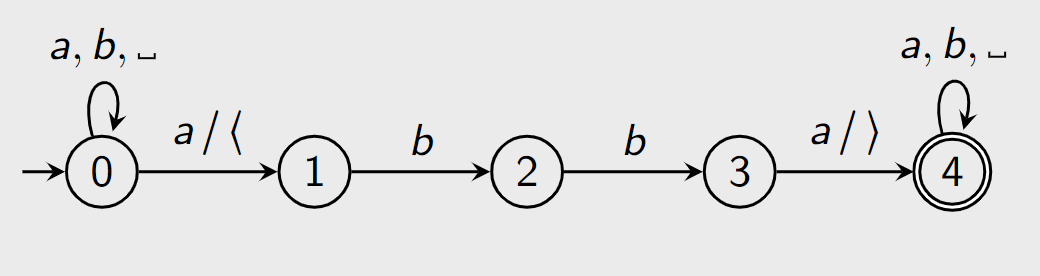
\includegraphics[scale=0.5]{img/cap6/ejemplo11_1.png}
        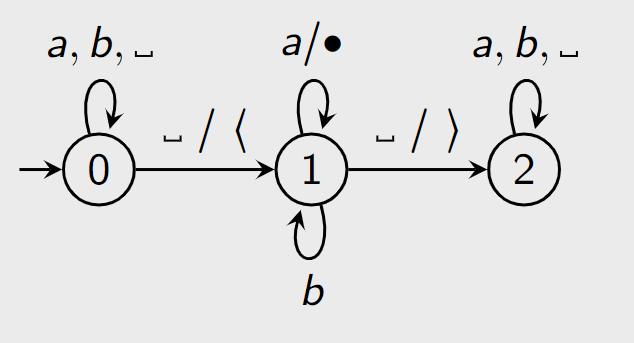
\includegraphics[scale=0.5]{img/cap6/ejemplo11_2.png}
    \end{figure}
}

\paragraph{Ejecución.} Sea un AnnA $\ca{N} = (Q, \Sigma, \Lambda, \Delta, I, F)$ y un documento $d = a_0 \ldots a_{n-1} \in \Sigma^*$. Una \textbf{ejecución} $\rho$ de $\ca{N}$ sobre $d$ es una secuencia:
$$
    \rho: p_0 \stackrel{t_0}{\rightarrow} p_1 \stackrel{t_1}{\rightarrow} \ldots \stackrel{t_{n-1}}{\rightarrow} p_n
$$
tal que cumple todas las siguientes condiciones:
\begin{enumerate}
    \item $p_0 \in I$
    \item para todo $i < n$, $t_i$ es de la forma $t_i = a_i$ o $t_i = (a_i, l)$ para algún $l \in \Lambda$
    \item para todo $i < n$, $(p_i, t_i, p_{i+1}) \in \Delta$
\end{enumerate}

Se define la \textbf{anotación de} $\rho$ como $\texttt{ann}(\rho) = \texttt{ann}_0(t_0) \cdot \ldots \cdot \texttt{ann}_n(t_{n-1})$:
$$
    \texttt{ann}_i(t)= \begin{cases}(i, l) & t=(a, l) \\ \epsilon & t=a\end{cases}
$$
Decimos que $\rho$ es de \textbf{aceptación} si, y sólo si, $q_n \in F$.

\ejemplo{Ejecuciones}{}{
    \vspace{-10pt}
    \img{img/cap6/ejemplo12.png}{0.55}

    Algunas ejecuciones sobre $d$:
    \begin{itemize}

        \item $\rho_1: p_0 \stackrel{a}{\rightarrow} p_0 \stackrel{\sbar / \langle}{\rightarrow} p_1 \stackrel{a / \bullet}{\rightarrow} p_1 \stackrel{b}{\rightarrow} p_1 \stackrel{b}{\rightarrow} p_1 \stackrel{a / \bullet }{\rightarrow} p_1 \stackrel{\sbar / \rangle}{\rightarrow} p_2 \stackrel{b}{\rightarrow} p_2 \stackrel{a}{\rightarrow} p_2 \stackrel{\hphantom{a}\sbar\hphantom{a}}{\rightarrow} p_2 \stackrel{b}{\rightarrow} p_2$

        \item $\rho_2: p_0 \stackrel{a}{\rightarrow} p_0 \stackrel{\hphantom{a}\sbar\hphantom{a}}{\rightarrow} p_0 \stackrel{a}{\rightarrow} p_0 \stackrel{b}{\rightarrow} p_0 \stackrel{b}{\rightarrow} p_0 \stackrel{a}{\rightarrow} p_0 \stackrel{\sbar / \langle}{\rightarrow} p_1 \stackrel{b}{\rightarrow} p_1 \stackrel{a / \bullet}{\rightarrow} p_1 \stackrel{\sbar / \rangle}{\rightarrow} p_2 \stackrel{b}{\rightarrow} p_2$
    \end{itemize}
    Además, tenemos que:
    \begin{itemize}
        \item $\texttt{ann}\left(\rho_1\right)=(1,\langle)(2, \bullet)(5, \bullet)(6,\rangle) \qquad \qquad a \, \overset{\langle}{\sbar} \, \overset{\bullet}{a}\, b\, b\, \overset{\bullet}{a}\, \overset{\rangle}{\sbar}\, b\, a\, \sbar \, b$

        \item $\texttt{ann}\left(\rho_2\right)=(6,\langle)(8, \bullet)(9,\rangle) \qquad \qquad \qquad a \, \sbar \, a \, b \, b \, a \, \overset{\langle}{\sbar} \, b \, \overset{\bullet}{a} \, \overset{\rangle}{\sbar} \, b $
    \end{itemize}
}

\paragraph{Output de un AnnA.} Sea $\ca{N}$ un AnnA. Se define la función $\llbracket \mathcal{N} \rrbracket$ tal que para todo documento $d \in \Sigma^*$:
\alignformula{
    \llbracket\mathcal{N} \rrbracket(d)=\{\texttt{ann}(\rho) \mid \rho \text { es una ejecución aceptación de } \mathcal{N} \text { sobre } d\}
}

\newpage

\ejemplo{Output de un AnnA}{}{
    \vspace{-10pt}
    \img{img/cap6/ejemplo12.png}{0.55}

    Para el documento $d$ se tiene que:
    $$
        \llbracket\mathcal{N}\rrbracket(d)=\{(1,\langle)(2, \bullet)(5, \bullet)(6,\rangle),(6,\langle)(8, \bullet)(9,\rangle)\}
    $$
}

\subsubsection{Desde un vset a AnnA}

\teorema{}{}{
    Sea $\Sigma$ un alfabeto finito. Para todo vset autómata funcional $\ca{A}$ sobre $\Sigma$, existe un AnnA $\ca{N}$ sobre $\Sigma \cup \{\#\}$ tal que para todo documento $d$ sobre $\Sigma$:
    $$
        \llbracket\mathcal{N} \rrbracket(d \cdot \#)=\{\operatorname{seq}(\mu) \mid \mu \in \llbracket \mathcal{A} \rrbracket(d)\}
    $$
}

El teorema anterior nos dice que $\ca{N}$ entrega la \textbf{secuenciación} de los mappings en $\llbracket \mathcal{A} \rrbracket(d)$.

\paragraph{Propiedades.} Sea $\ca{A} = (Q, \Sigma, \ca{X}, \Delta, I, F)$ un vset autómata funcional y $p,q \in Q$. \textbf{Sin pérdida de generalidad}, desde ahora supondremos que todos los estados de un vset autómata funcional $\ca{A}$ son \textbf{útiles}. En otras palabras, para todo estado $p \in Q$ de $\ca{A}$:
\begin{itemize}
    \item Existe una ejecución (camino de transiciones) desde $I$ a $p$.
    \item Existe una ejecución (camino de transiciones) desde $p$ a $F$.
\end{itemize}

\paragraph{Definición.} Una \textbf{ejecución sin lectura} (ejec-SL) de $p$ a $q$ en $\ca{A}$ es una secuencia:
$$
    \pi: \quad p_0 \stackrel{s_0}{\rightarrow} p_1 \stackrel{s_1}{\rightarrow} \ldots \stackrel{s_{k-1}}{\rightarrow} p_k
$$
donde:
\begin{itemize}
    \item $p_0 = p$ y $p_k = q$
    \item para todo $i < k$, $(p_i, s_i, p_{i+1})$ y $s_i \in \texttt{Markers}(\ca{X}) \cup \{\epsilon\}$.
\end{itemize}

Una ejecución sin lectura es un \textbf{camino de transiciones} de $p$ a $q$ tal que $s_i \notin \Sigma$. También, definimos el \textbf{conjunto de} $\pi$ como
$$
    \texttt{set}(\pi) = \{ s_i \mid s_i \in \texttt{Markers}(\ca{X})\}
$$

\paragraph{Propiedades ejec-SL.} Tenemos que:
\begin{enumerate}
    \item Para todo $i \neq j$, si $s_i = s_j$, entonces $s_i = s_j = \epsilon$.
    \item Para todo par de ejec-SL distintas $\pi_1, \pi_2$ de $p$ a $q$ en $\ca{A}$, se cumple que $\texttt{set}(\pi_1) = \texttt{set}(\pi_2)$.
\end{enumerate}

La demostraciones de estas propiedades queda como ejercicio propuesto para el lector.

\newpage

\paragraph{Demostración teorema 33.} Dado un vset autómata funcional $\ca{A} = (Q, \Sigma, \ca{X}, \Delta, I, F)$, construimos:
$$
    \mathcal{N}=\left(Q, \Sigma \cup\{\#\}, 2^{\texttt{Markers }(\mathcal{X})}, \Delta^{\prime}, I, F\right)
$$
\begin{multicols}{2}
    $(p,a,q) \in \Delta'$ $\Leftrightarrow$ existe $p' \in Q$ y una ejec-SL $\pi$ de $p$ a $p'$ tal que $(p',a,q) \in \Delta$ y $\texttt{set}(\pi) = \varnothing$.
    \img{img/cap6/teo_1.png}{0.2}

    $(p,a,S,q) \in \Delta'$ $\Leftrightarrow$ existe $p' \in Q$ y ejec-SL $\pi$ de $p$ a $p'$ tal que $(p',a,q) \in \Delta$ y $\texttt{set}(\pi) = S \neq \varnothing$.
    \img{img/cap6/teo_2.png}{0.2}

    $(p,\#, q) \in \Delta'$ $\Leftrightarrow$ existe una ejec-SL $\pi$ de $p$ a $q$ tal que $\texttt{set}(\pi)=\varnothing$ y $q \in F$
    \img{img/cap6/teo_3.png}{0.2}

    $(p,\#, S, q) \in \Delta'$ $\Leftrightarrow$ existe una ejec-SL $\pi$ de $p$ a $q$ tal que $\texttt{set}(\pi)=S \neq \varnothing$ y $q \in F$
    \img{img/cap6/teo_4.png}{0.2}
\end{multicols}
Por las propiedades 1 y 2, la construcción es \textbf{correcta}. Por último, podemos ver que
$$
    \llbracket \mathcal{N} \rrbracket(d \cdot \#)=\{\texttt{seq}(\mu) \mid \mu \in \llbracket \mathcal{A} \rrbracket(d)\}
$$
\hfill $\blacksquare$

\ejemplo{Construcción}{}{
    \img{img/cap6/ejemplo14.png}{0.5}
}

\newpage

\subsubsection{Determinismo}

Sea $\ca{N} = (Q,\Sigma, \Lambda, \Delta, I, F)$ un autómata con anotaciones AnnA.

\paragraph{Definición.} Decimos que $\ca{N}$ es \textbf{Input-Output} determinista (I/O-determinista) si, y sólo si, $|I| = 1$ y para todo $\left(p, t_1, q_1\right),\left(p, t_2, q_2\right) \in \Delta$, si $t_1 = t_2$, entonces $q_1 = q_2$. \bigbreak

$\ca{N}$ funciona de manera determinista al recibir el documento y una \textbf{anotación simultáneamente}.

\ejemplo{}{}{
    \begin{figure}[H]
        \centering
        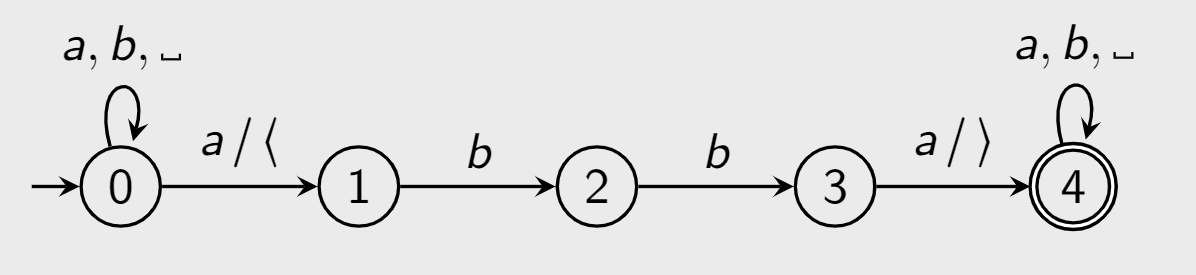
\includegraphics[scale=0.5]{img/cap6/ejemplo15_1.png}
        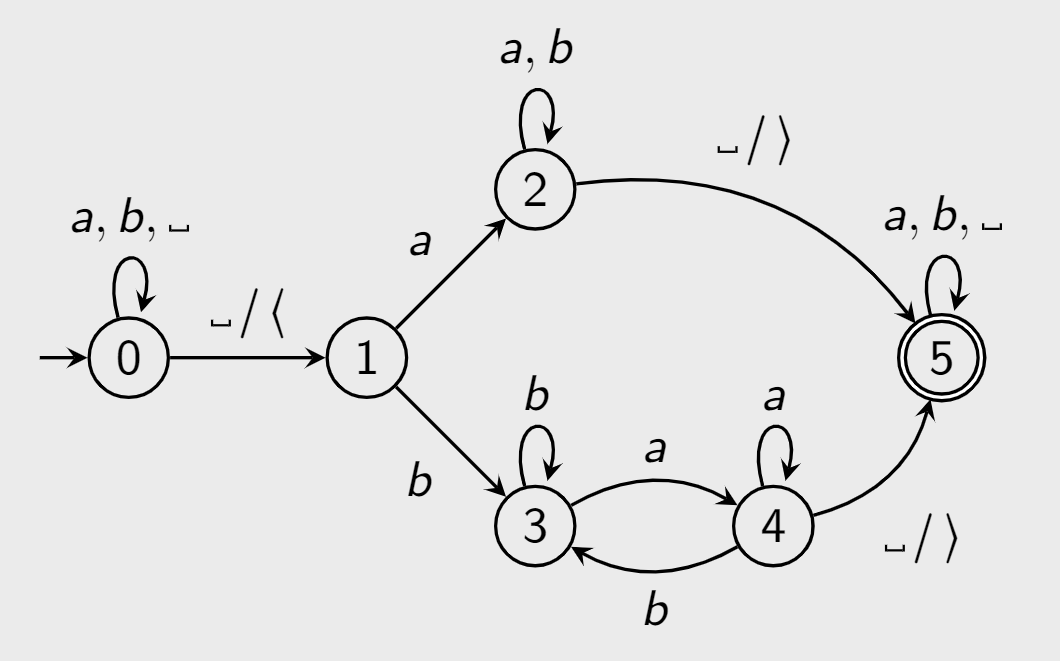
\includegraphics[scale=0.5]{img/cap6/ejemplo15_2.png}
    \end{figure}
}

\teorema{}{}{
Para todo AnnA $\ca{N} = (Q, \Sigma, \Lambda, \Delta, I, F)$, existe un AnnA I/O-determinista $\ca{N}^\text{det}$ tal que
$$
    \llbracket \mathcal{N} \rrbracket=\llbracket \mathcal{N}^{\text {det}} \rrbracket
$$
}

\paragraph{Demostración teorema 34.} Considere la determinización de $\ca{N}$ como:
$$
\mathcal{A}^{\text{det}}=\left(2^Q, \Sigma, \Lambda, \Delta^{\text{det}}, q_0^{\text{det}}, F^{\text{det}}\right)
$$
donde:
\begin{itemize}
    \item $2^Q=\{S \mid S \subseteq Q\}$ es el conjunto potencia de $Q$.
    \item $q_0^{\text{det}}=I$
    \item $\Delta^{\operatorname{det}}: 2^Q \times(\Sigma \cup \Sigma \times \Lambda) \rightarrow 2^Q$ tal que para todo $t \in \Sigma \cup(\Sigma \times \Lambda)$:
    $$
    \Delta^{\text{det}}(S, t)=\{q \in Q \mid \exists p \in S.\ (p, t, q) \in \Delta\}
    $$
    \item $F^{\text{det}}=\left\{S \in 2^Q \mid S \cap F \neq \varnothing\right\}$.
\end{itemize}









